\chapter{XML protokol}
\label{kap_xml}
Pan Ing. Peter Macejko ve své diplomové práci navrh systém vzdálené správy strojů pomocí komunikačního protokolu, využívajícího XML. V této kapitole budou shrnuty všechny 
navržené postupy od mapování SNMP informačního modelu až po komunikační struktury využívané správcem a spravovanými zařízeními.

\section{Obecný informační model}
Informační model je nedílnou součástí celého systému správy dat. Do něj jsou mapována veškerá monitorovaná data a jsou zde i vyjádřeny vztahy mezi daty. Ve skutečnosti
omezuje počet a druh možných dotazů. Výsledný systém, který byl pro popis jednotlivých zařízení navržen vychází z několika různých přístupů abstrakce a popisu dat.

Nejprve byla analýza problému založena na dvou možnostech - přímém mapování MIB stromu do XML dokumentu, kdy by jednotlivé uzly přesně odpovídaly MIB struktuře; objektově
orientovaném využívajícím objektové paradigma. První přístup má výhodu ve snadném převodu MIB databáze do nového formátu, ale naopak ztrácí výhodu snadné rozšiřitelnosti,
která je vlastní XML technolgoii. Problém objektového mapování je nejednoznačné rozmístění uzlů ve stromu na objekty. Takovéto mapování by bylo nutno provádět
neautomatizovaně, tj. s dopomocí člověka.

Výsledkem analýzy problému je systém využívající kousek od obou přístupů. Na nejvyšší úrovni abstrakce je každé zařízení složeno z modulů. Každý model obsahuje jistou
funkcionalitu, která je úplně oddělena od těch zbývajících. Mezi tyto moduly patří i v této práci navrhovaná brána, která propojuje zařízení bez XML podpory s ostatními
částmi sítě. V této chvíli se jedná pouze o obecný návrh každého zařízení.

\subsection{Odvození typů}
Odvozování typů je založeno na principu dědičnosti. Definice jako takové jdou od abstraktního až po detailní popis.

\subsection{Definice modulů}
Jak již bylo řečeno, každé zařízení se skládá z modulů. Jednotlivé moduly jsou též popsány XML schématem. Každé takové schéma
musí splňovat přesné požadavky na poskytované informace.

Musí být detailně popsána funkčnost, přiděleno unikátní jméno, typ a cesta ve stromové struktuře, použitá pro adresaci jednotlivých uzlů. 
SNMP moduly mají definován kořenový element, který je využit pro spojování více MIB informačních bází dohromady.

Přesný popis je možné nalézt v \cite{macejko_dipl} v kapitole 5.2.3.
%TODO doplnit citaci dle normy

\subsection{Popis zařízení}
Pro popis zařízení je využito XML schéma, stejně jako pro popis dalších částí (modulů, apod.). Na obrázku \ref{obr_xml_popis_zarizeni} je znázorněno,
jak vypadá zařízení popsané od nejvyšší úrovně. 

\begin{figure}[htp]
	\begin{center}
		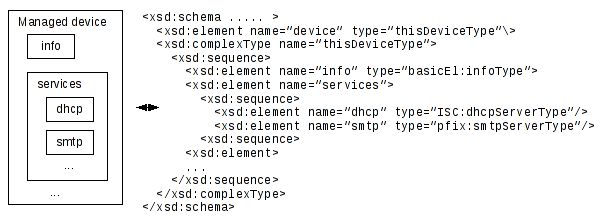
\includegraphics[width=15cm]{obrazky/03_popis_zarizeni.png}
		\caption{Popis zařízení v XML schématu (obrázek 5.8, \cite{macejko_dipl})}
		\label{obr_xml_popis_zarizeni}
	\end{center}
\end{figure}

\subsection{Oznamovací zprávy}
Oznámení jsou takové zprávy, které jsou zasílány manažerovi v případě, že se na monitorovaném zařízení vyskytne nějaká událost (shodné s SNMP Trap zprávami).
V rámci SNMP jsou tyto zprávy součástí datového modelu, nicméně tyto specifické uzly MIB stromu nenesou žádná data a jsou tudíž použité pouze při generování typu
chyby či události. 

V navrženém systému jsou všechny možné upozornění (ať již předdefinované, či definované administrátorem) umístěny ve speciálním uzlu stromu \verb|notifications|, 
kde je velice jednoduché dohledat, jaké události mohou způsobit zaslání oznamuvací zprávy. Každý modul pak může mít specifikován speciální typ \verb|NotificationType|,
který popisuje právě onu událost.

\subsection{Adresace dat}
Pro adresaci dat je možno využít postupů XPath a XQuery. Jednotlivými výrazy ať už v jednom či druhém případě se bude manažer dotazovat na jednotlivé uzly v
rámci spravované databáze.


\section{Mapování MIB do XML}
V předchozí části byl rozebrán čistě obecný model popisu zařízení. Pro monitorované stroje, které nejsou kompatibilní s XML protokolem, musí existovat brána,
která bude překládat dotazy z jednoho protokolu na druhý a stejně tak i odpovědi. Je tedy nutné přesně definovat postup přepisu MIB na XML.

Je nutné vyřešit tři základní problémy - jak vyřešit importy jednotlivých MIB do sebe; jak předefinovat datové typy a jak konvertovat celý MIB strom.

\subsection{Importy}
V rámci jednotlivých MIB jsou časté odkazy na báze vyšší úrovně, kdy pak na nižších úrovních definujeme jenom část podstromu. V rámci XML budou definovány 
odkazy jako prostory jmen, které jsou odvozeny od názvu daného MIB. Odkaz na jiné schéma bude proveden použitím odkazů na typ s příslučným názvem prostoru jmen. 

\subsection{Datové typy}
V SNMP, jak bylo řečeno v předchozí kapitole, existuje několik druhů datových typů. Jednoduché (integer, string,...), aplikačně rozšířené (Gauge, IpAddress,...) a 
uživatelem definované.

Jednoduché typy budou mapovány na jejich XML ekvivalent. Na obrázku \ref{obr_xml_smi1_typy} je soupis všech aplikačně rozšířených typů a jejich popis
pomocí XML schématu (v rámci standardu SMIv1).

\begin{figure}[htp]
	\begin{center}
		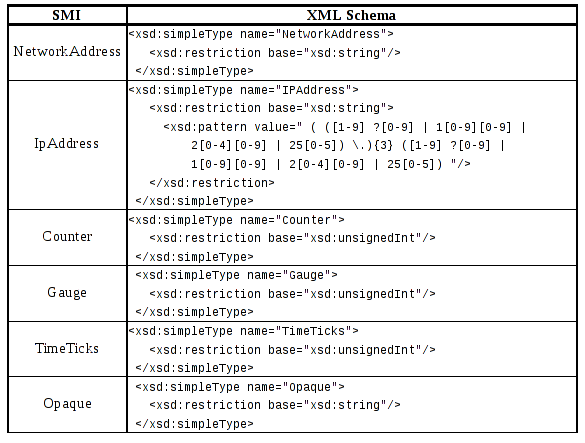
\includegraphics{obrazky/03_mapovani_smiv1.png}
		\caption{Mapování aplikačních typů SMIv1 do XML schématu (obrázek 5.2, \cite{macejko_dipl})}
		\label{obr_xml_smi1_typy}
	\end{center}
\end{figure}

\begin{table}
	\centering
	{\footnotesize
	  \begin{tabular}{|p{15cm}|}
      \hline
\begin{verbatim}...
    <xsd:element name="NodeName" type="MIBName:NodeNameType"/>
...
<xsd:simpleType name="NodeNameType">
  <xsd:annotation>
    <xsd:documentation xml:lang="en">DescrText</xsd:documentation>
    <xsd:appinfo>
      <status>StatusType</status>
      <access>AccessType</access>
      <oid>AbsoluteOID</oid>
    </xsd:appinfo>
  </xsd:annotation>
  <xsd:restriction base="NodeType"/>
</xsd:simpleType>\end{verbatim}\\
      \hline
    \end{tabular}
  }
	\caption{Mapování makra OBJECT-TYPE, jednoduchý typ (SMIv1) (tabulka 5.6, \cite{macejko_dipl})}
	\label{tab_xml_smi1_simple_type}
\end{table}

Součástí SMI je i možnost definovat vlastní typy. I pro tyto případy je nutno uvést definici překladu. Existují tři základní omezení při vytváření vlastních typů -
výčet, délka řetězce a rozmezí hodnot. Všechny tyto typy jsou detailně popsány a vyobrazeny v \cite{macejko_dipl}, kapitola 5.3.1.

\subsection{MIB strom}
Navržený systém využívá při mapování celého stromu oddělení definicí typů od samotné struktury stromu. Typy jsou definovány globálně a zároveň separátně od 
struktury a to z důvodu možného použití typů v rámci jiného modulu a zároveň při omezení přístupových práv do danéh oblasti stromu. V MIB jsou objekty
definovány makry (specifikované v SMI), které popisují několik základních typů uzlů. SMIv1 specifikuje OBJECT-TYPE a TRAP-TYPE makra.

OBJECT-TYPE makro definuje uzel, který obsahuje nějaká data. Může to být samotná hodnota, položka, nebo celá řádka tabulky. Mapování pak závisí na
položce \verb|SyntaxType| v samotné definici makra.

Pakliže je hodnota položky základním, rozšířeným či uživatelsky definovaným typem, bude vytvořena globální definice typu a položka bude tvořena elementem
s jednoduchým typem. Schematicky vyjádřeno v tabulce \ref{tab_xml_smi1_simple_type}.

Jestli bude hodnotou \verb|SEQUENCE|, bude vytvořen "řádkový" typ (tabulka \ref{tab_xml_smi1_sequence}).

Hodnota \verb|SEQUENCE OF| pak vyjadřuje množinu řádkových typů (tabulka \ref{tab_xml_smi1_sequenceof}).


\begin{table}
	\centering
	{\footnotesize
	  \begin{tabular}{|p{15cm}|}
      \hline
\begin{verbatim}...
    <xsd:element minOccurs="0" maxOccurs="unbounded"
             name="NodeName" type="MIBName:NodeNameType"/>
...
<xsd:complexType name="NodeNameType">
  <xsd:sequence>
    <xsd:element name="..child.." type="..childType.."/>
    ...
  </xsd:sequence>
</xsd:complexType>\end{verbatim}\\
      \hline
    \end{tabular}
  }
	\caption{Mapování SEQUENCE, makro OBJECT-TYPE (tabulka 5.7, \cite{macejko_dipl})}
	\label{tab_xml_smi1_sequence}
\end{table}

\begin{table}
	\centering
	{\footnotesize
	  \begin{tabular}{|p{15cm}|}
      \hline
\begin{verbatim}...
  <xsd:element name="atTable">
    <xsd:complexType>
      <xsd:sequence>
        <xsd:element ..SEQUENCE.. />
      </xsd:sequence>
    </xsd:complexType>
  </xsd:element>
...\end{verbatim}\\
      \hline
    \end{tabular}
  }
	\caption{Mapování SEQUENCE OF, makro OBJECT-TYPE (tabulka 5.8, \cite{macejko_dipl})}
	\label{tab_xml_smi1_sequenceof}
\end{table}

Dalším typem objektu jsou upozornění definované pomocí TRAP-TYPE makra. Tyto definují uzly bez hodnot, pouze specifikují danou událost. V navrženém systému
tedy nemusí být součástí stromu, ale pouze globálních typových definicí. Bude použit jednoduchý typ popisující čas a den (datetime type) se speciálním elementem
v části \verb|appinfo|.

\begin{table}
	\centering
	{\footnotesize
	  \begin{tabular}{|p{15cm}|}
      \hline
\begin{verbatim}<xsd:simpleType name="NodeNameType">
  <xsd:annotation>
    <xsd:documentation xml:lang="en">DescrText</xsd:documentation>
    <xsd:appinfo>
      <enterprise>EnterpriseName</enterprise>
      <variable>VariableType</variable>
      <reference>ReferenceType</reference>
      <trapNumber>TrapNumber</trapNumber>
    </xsd:appinfo>
  </xsd:annotation>
  <xsd:restriction base="xsd:dateTime"/>
</xsd:simpleType>\end{verbatim}\\
      \hline
    \end{tabular}
  }
	\caption{Mapování TRAP-TYPE makra (tabulka 5.10, \cite{macejko_dipl})}
	\label{tab_xml_trap_type}
\end{table}

\newpage

\section{Zprávy}


